\section{Specific Object Recognition}

A specific object = an instance of an object class e.g. “my car” instead of “a car”

Must overcome:
\begin{itemize}
	\item Illumination
	\item Object pose
	\item Clutter
	\item Occlusions
	\item Viewpoint
\end{itemize}

For class recognition also intra-class variation must be detected.

\subsection{Model based}
comparing image features with features of objects in a database, trying to figure out type + pose

this is SLOW and especially the need to get both object type and pose
right to formulate a correct hypothesis is problematic

\subsubsection{Invariant-based recognition of planar shapes}
The crucial advantage of invariants is that they decouple object type and pose issues

ratios of areas
are affine invariant and the following invariants are based on this

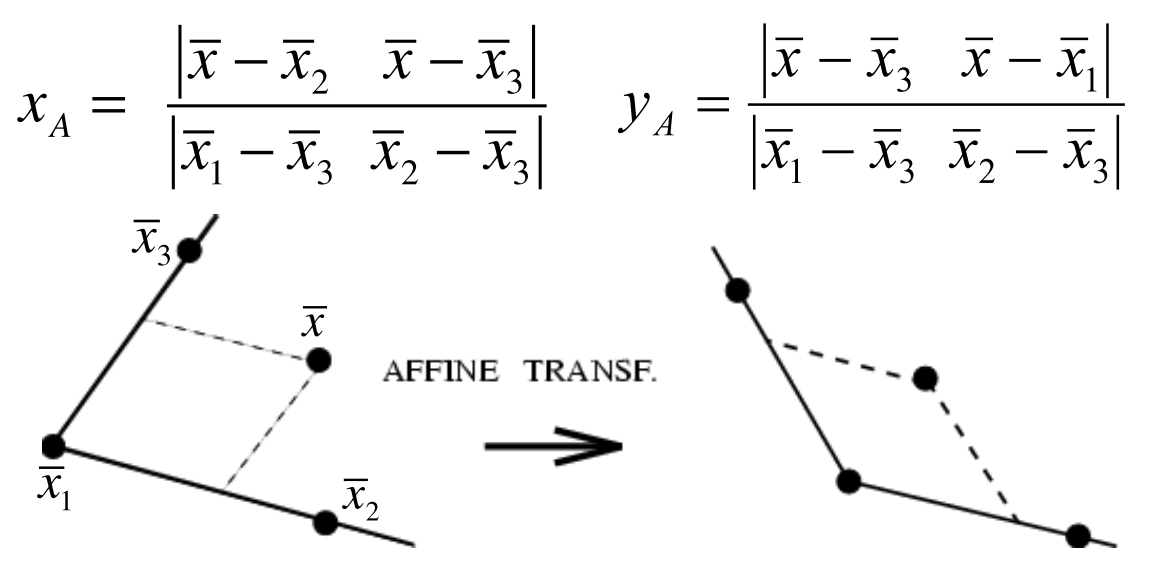
\includegraphics[width=\columnwidth]{pictures/affine}

\subsection{Image based}
PCA represents data in a lower-dimensional space keeping most of the variance
It was seen to be powerful for similar patterns like faces, that exhibit a lot of redundancy

\subsubsection{Appearance manifold approach}
Training:\\
for every object : - sample the set of viewing conditions (mainly viewpoints in this ex.)
- use these images as feature vectors (after manual bounding-box fitting around the object, rescaling, brightness normalization)
over all objects: - apply a PCA over all the images of all objects (directly on the images)
- keep the dominant PCs (10-20 enough already)
- sequence of views for 1 object represent a manifold in the space of projections (fit splines to manifolds + resample if desired)

Recognition stage (aka `Testing’)\\

Represent the incoming image as a point in the same PC space
Type: what is the nearest manifold to the point ?
Pose: what is the closest point on that closest manifold ?

\subsection{Model based vs appearance based}
Model vs Image\\

+Compact model vs -Large models
+Can deal with clutter vs -Cannot deal with clutter
-Slow analysis-by-synthesis vs +Efficient
-Models difficult to produce vs +Models easy to produce
-For limited object classes vs +For wide classes of objects

\subsection{Hybrid techniques}
\subsubsection{Euclidean invariant feature}

Training
\begin{enumerate}
	\item look for corners (with the Harris corner detector)
	\item  take circular regions around these points, of multiple radii (cope a bit with scale changes)
	\item calculate from the intensities in the circular regions . invariants under planar rotation -> feature vectors
	\item do this from different viewpoints, where the invariance cuts down on the number of views needed (here no in-plane rotations necessary)
	\item put for every object and for each of its viewpoints the . list of corner positions and their invariant feature . vectors (descriptors) in a database
\end{enumerate}

Testing
\begin{enumerate}
	\item extract corners and their invariant descriptors from the incoming image
	\item compare these invariants with those stored in the database -> find matches
	\item look for consistent placement of candidate matching corner points (e.g. using epipolar geometry)
	\item decide which object based on the number of remaining matches (i.e. consistently placed matches) (the best matching image yields the object type+appr.pose)
\end{enumerate}

\subsubsection{Recognition using local affine and photometric invariant features}
Invariant features = features that are preserved under a specific group of transformations\\



hyprid approach that aims to deal with large variations in
\begin{itemize}
	\item Viewpoint
	\item Illumination
	\item Background
	\item Occlusions
\end{itemize}





